\section{DBT}\label{Appendix:DBT}
La principal complicación del desarrollo de una red distribuída basada en el BUS
CAN, es que puedan comunicarse correctamente entre sí, cómo se deben asignar
los identificadores (Node-ID) correctamente a cada uno de los nodos y cómo se
asignan los tiempos de inhibición. Los Node-ID y los tiempos de inhibición se
deben distribuir entre los nodos de tal manera de asegurar que:
\begin{itemize}
\item Se preveean los conflictos entre nodos. Por ejemplo diferentes funciones
  que usan el mismo identificador.
\item Se preveean la falta de coincidencia. Por ejemplo que existan diferentes
  indentificadores para el mismo nodo.
\item ofrecer el control integrado para un comportamiento dinámico del
  sistema.  
\end{itemize}

El protocolo CAN (CAN Application Layer for Industrial Applications
CiA/DS204-1) dispone la existencia de 3 métodos para distribuir identificadores
y tiempo de inhibición a un módulo.

\begin{itemize}
\item \textbf{Distribución estándar}: en este método los identificadores y
  tiempos de inhibición son estandarizados por el módulo proveedor (nodo
  monitor. Una distribución estándar require la estandarización de todas las
  funciones y su correspondiente identificador.
\item \textbf{Distibución estática}: En este método los identificadores y los
  tiempos de inhibición son fijos. Todos los identificadores y los tiempos de
  inhibición son fijados en el momento del desarrollo.
\item \textbf{Distribución dinámica}: En este método los identificadores y los
  tiempos de inhibición son distribuidos vía red CAN a través del servicio
  estándar y un protocolo definido.  
\end{itemize}

En esta instancia de trabajo, para el desarrollo del protocolo CANae, se utilizó
el \textit{método de distribución estática}. Esto exige que los nodos ya cuenten
con un identificador y tiempos de inhibición por defecto. Esto se asigna en el
momento del desarrollo del diseño e ingeniería de la arquitectura de aviónica.
Esto reduce considerablemente la complejidad de la entidad DBT. Si bien
originalmente, el DBT es un elemento de servicio de la capa de aplicación CAN
que ofrece una distribución dinámica de identificadores y tiempos de inhibición,
en CANae es utilizado para asegurar la correcta comunicación y consistencia de
los nodos y la red en su conjunto.

La arquitectura del DBT se puede observar en la Figura \ref{fig:DBT}

\begin{figure}[h!]
 \centering
 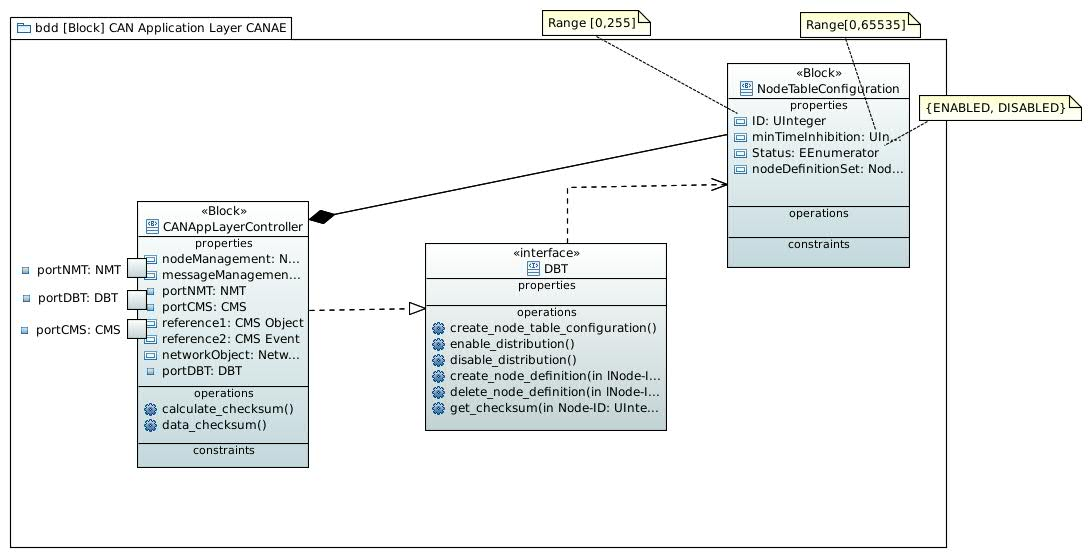
\includegraphics[scale=0.4]{images/Secciones/AppendixA/DBT.JPG}
  \caption{Arquitectura de la entidad DBT}
\label{fig:DBT}
\end{figure} 

\subsection{Objetos y servicios de DBT}
El DBT de CANae utiliza 2 objetos para modelar su funcionamiento:
\begin{itemize}
\item \textbf{Node-ID Database (NodeTableConfiguration)}: Esta tabla contiene la
  definición de todos los nodos conectados a la red. Esta tabla está compuesta
  por Node-ID Definitions
\item \textbf{Node-ID Definition}: define todos los atributos de un Node-ID.
  Contiene una definición de usuario creado por el usuario.
\end{itemize}

El DBT de CANae ofrece las siguientes categorias de servicio:
\begin{itemize}
\item \textbf{Distribution Control Services}: esta es tarea del nodo monitor de
  enviar el identificador y los tiempos de inhibición a todos los nodos
  conectados a la red. Los datos que son enviados por el nodo monitor son
  corroborados por los nodos, comprobando que el ID enviado coincida con su
  propio Node-ID.
\item \textbf{Consistency Control Services}: através de este servicio cada nodo
  puede detectar inconsistencia en el NodeTableConfiguration e inconsistencia
  entre nodos.
\end{itemize}

\subsection{Descripción de los servicios DBT}
Los servicios se describen en forma de tabla que contiene los parámetros de
cada función que se define para ese servicio. Los parámetros determinan el tipo
de servicio.  Todos los servicios asumen que no ocurrieron ningún tipo de error
en la capa de física ni en la capa de enlace de datos.

\subsection{Objetos DBT}
Los objetos que utiliza la entidad DBT para modelar el servicio son los
siguientes:
\begin{itemize}
\item \textbf{Node Table Configuration (Node-ID Database)}
  \begin{itemize}
  \item \textbf{Atributos}
    \begin{itemize}
    \item \underline{Estado}: Uno de los valores {ENABLED, DISABLED}. Este
      atributo indica si el DBT Monitor es capaz de distribuir los Node-ID
      y tiempos de inhibición. En esta instancia de trabajo el valor del estado
      en el DBT del Nodo Monitor será DSIABLED
      \item \underline{Node Definition Set} set de todas las definciones. 
    \end{itemize}
  \end{itemize}

\item \textbf{Node-ID Defintion}:
  Las definciones contiene los siguientes datos:
  \begin{itemize}
  \item \underline{ID}: Valor en el rango de [0,255]
  \item \underline{Mínimo tiempo de inhibición}: en el rango [0,65535] indicando
    el valor mínimo en unidades de 100$\mu$sec para el tiempo de inhibición.
  \end{itemize}
  
\end{itemize}

\subsection{Servicios DBT}\label{subsection:servicios_dbt}
\subsubsection{Distribution Control Services}
\begin{itemize}
  \item create\_node\_table\_configuration()
  \item enable\_distribution()
  \item disable\_distribution()
  \item create\_node\_definition(UInteger lNode-ID, UInteger hNode-ID, UInteger minInhibitTime)
    \begin{itemize}
    \item \textbf{UInteger lNode-ID}: Límite inferior del rango de IDs.
    \item \textbf{UInteger hNode-ID}: Límite superior del rango de IDs.
    \item \textbf{UInteger minInhibitTime}: Tiempo mínimo de inhibición de cada
      nodo.
    \end{itemize}
  \item delete\_node\_definition(UInteger lNode-ID, UInteger hNode-ID)
\end{itemize}

\subsubsection{Consistency Control Service}

\begin{itemize}
\item get\_checksum(UInteger Node-ID, Float checksum)
  \begin{itemize}
      \item \textbf{UInteger Node-ID}: ID del nodo que desea controlar la
    consistencia.
      \item \textbf{UInteger checksum}: checksum de la DBT Definition.
  \end{itemize}
\end{itemize}


\subsection{Protocolos DBT}
\subsubsection{Crear NodeTableConfiguration}
El La tabla de configuración del nodo juega un papel similar al que lo haría el
Node-ID DATABASE del estándar CAN. La principal diferencia, es que esta tabla
se encuentra presente en todos los nodo y no en el ``Master'', ya que este
protocolo está pensado para ser utilizado en redes distribuidas, donde no
existe un nodo central o master.

El nodo monitor envía la señal a los nodos de crear la tabla de configuración
del nodo através de \textit{create\_node\_table\_configuration()}. Este es
recibido através de la interfaz DBT del nodo, y crea el objeto
\textit{NodeTableConfiguration}. Esto se observa en la Figura
\ref{fig:createNodeTableConfiguration}.

\begin{figure}[h!]
 \centering
 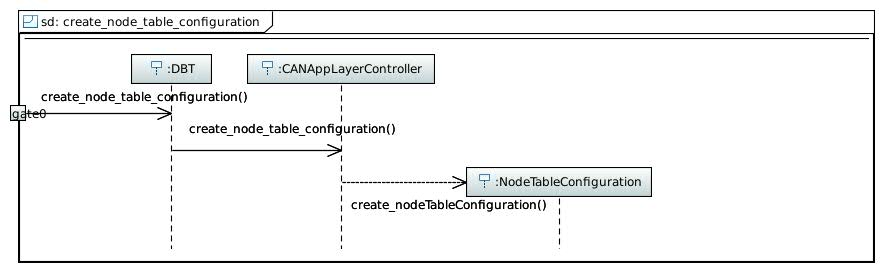
\includegraphics[scale=0.4]{images/Secciones/AppendixA/create_node_table_configuration.JPG}
  \caption{Protocolo create\_node\_table\_configuration}
\label{fig:createNodeTableConfiguration}
\end{figure} 

\subsubsection{Habilitar distribución}
La distribución de Node-ID es utilizada cuando se utiliza el método de
asignación dinámica. En esta versión del protocolo la distribución del ID se
encuentra desactivada. En la Figura \ref{fig:enable_distribution} se puede
obseevar el protocolo.

\begin{figure}[h!]
 \centering
 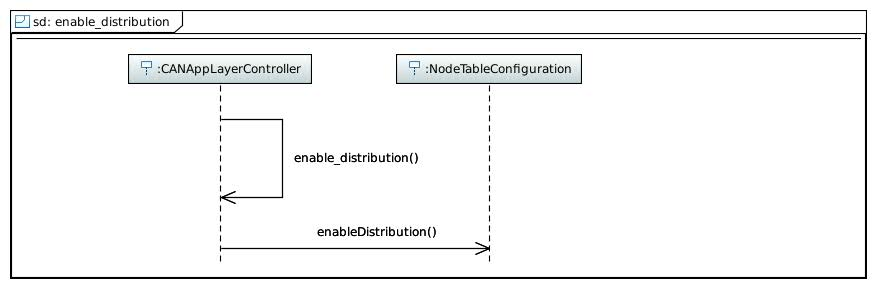
\includegraphics[scale=0.4]{images/Secciones/AppendixA/enableDistribution.JPG}
  \caption{Protocolo enable\_distribution}
\label{fig:enable_distribution}
\end{figure}

\subsubsection{Deshabilitar distribución}
Esta opción se encuentra por defecto en esta versión del protocolo CANae. El ID
se distribuye estáticamente. Son preestablecidos durante el desarrollo. En la
Figura \ref{fig:disable_distribution}

\begin{figure}[h!]
 \centering
 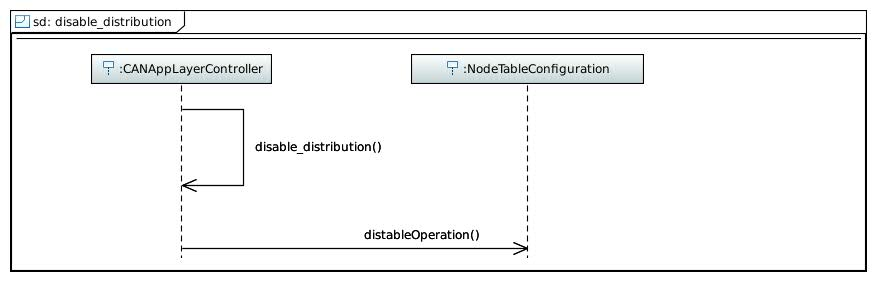
\includegraphics[scale=0.4]{images/Secciones/AppendixA/disable_distribution.JPG}
  \caption{Protocolo disable\_distribution}
\label{fig:disable_distribution}
\end{figure}


\subsubsection{Crear definición del nodo}
El nodo monitor envía la señal para que sea creen las definiciones de nodo. Para
ello es necesario que el nodo monitor envíe los rangos permitidos para la
definición de los nodos. Esto se define a través de las variables
\textit{lNode-ID} y \textit{hNode-ID}. En esta versión del protocolo estas
variables no son utilizadas ya que los Node-ID ya se encuentran definidas
estáticamente. También el nodo monitor envía el tiempo mínimo de inhibición
explicado anteriormente. El nodo monitor hace este proceso con todos los nodos
de la red a través del mensaje \textit{create\_node\_definition}. Este se lo
puede observar en la Figura \ref{fig:create_node_definition}.

\begin{figure}[h!]
 \centering
 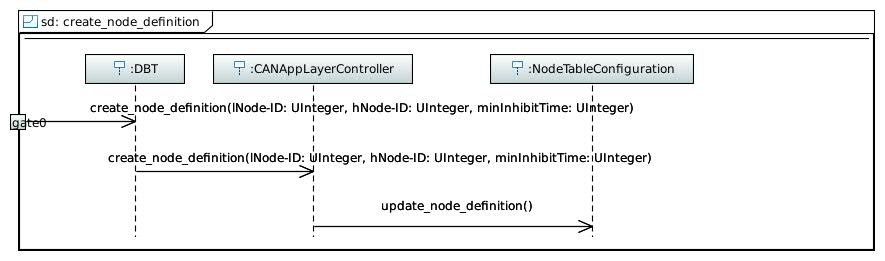
\includegraphics[scale=0.4]{images/Secciones/AppendixA/create_node_definition.JPG}
  \caption{Protocolo create\_node\_definition}
\label{fig:create_node_definition}
\end{figure}


\subsubsection{Eliminar la definición del nodo}
Esta función es utilizada para eliminar la definción del nodo. Se lleva a cabo
para eliminar un nodo de la red. Se hace através de la función
\textit{delete\_node\_definition()}. Esta se la puede observar en la Figura
\ref{fig:delete_node_definition}

\begin{figure}[h!]
 \centering
 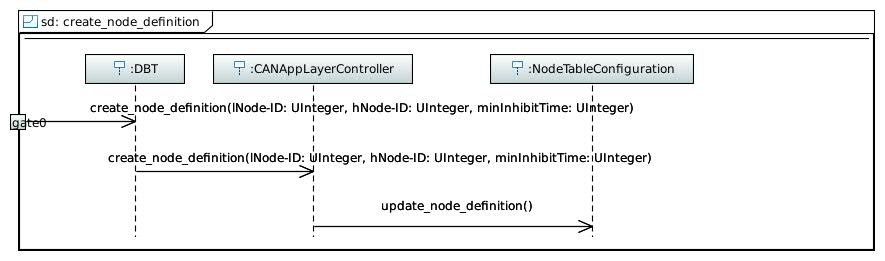
\includegraphics[scale=0.4]{images/Secciones/AppendixA/create_node_definition.JPG}
  \caption{Protocolo delete\_node\_definition}
\label{fig:delete_node_definition}
\end{figure}


\subsubsection{Checksum}
Para poder asegurar la integridad de los nodos conectados a la red, se puede
utilizar este mecanismo para comprobar de que la información, referente a
la definición de los nodos, se encuentra correctamente en todos los nodos. Para
ello, cada nodo lleva a cabo un checksum de su información y la envía por la
red. Como esta está basada en el Bus-CAN, el mensaje llega correctamente a todos
los nodos. Los nodos realizan sus comprobaciones y responden. Si la información
es correcta deben responder con un mensaje que contegan bits NO dominantes. En
el caso de que se produzca alguna diferencia en los checksum deberán responder
con bits dominantes. Cuando esto se produzca deberán llevarse a cabo medidas de
recuperación o reconfiguración de la red. Este protocolo se lo puede observar en
la Figura \ref{fig:get_checksum}

\begin{figure}[h!]
 \centering
 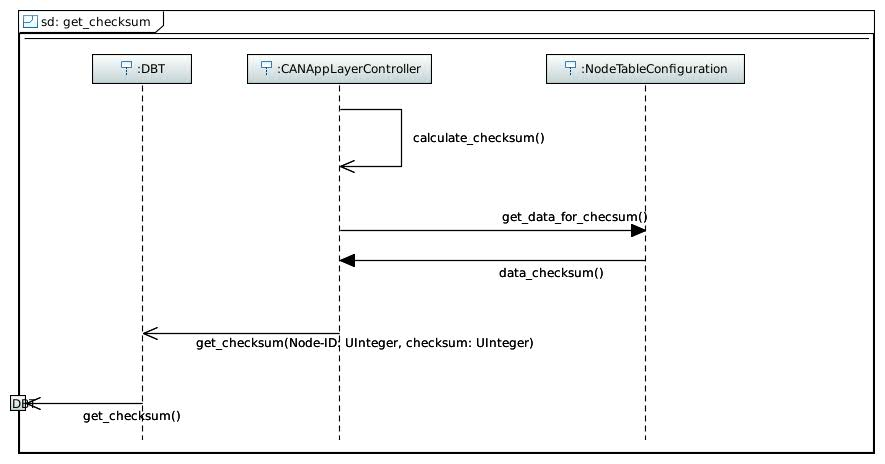
\includegraphics[scale=0.4]{images/Secciones/AppendixA/get_checksum.JPG}
  \caption{Protocolo get\_checksum}
\label{fig:get_checksum}
\end{figure}

